\begin{center}
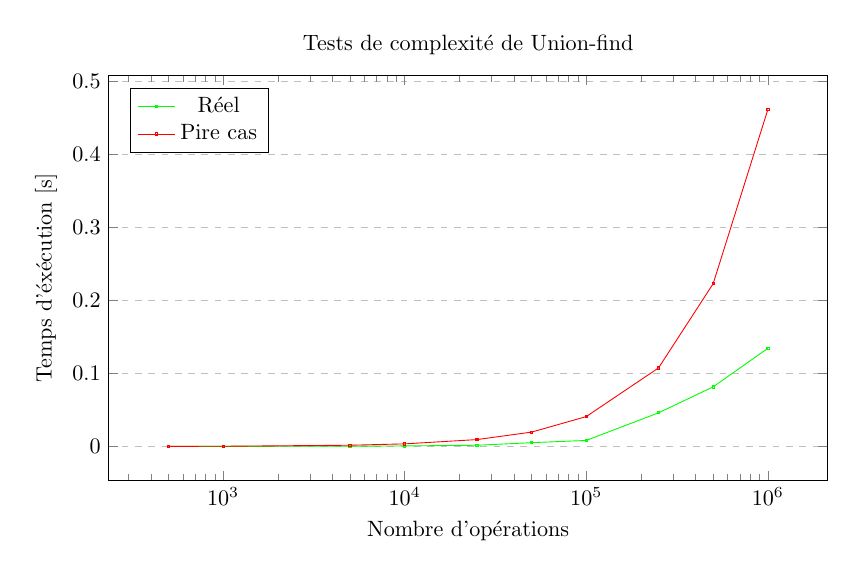
\begin{tikzpicture}[scale=0.8]
\begin{axis}[
    title={Tests de complexité de Union-find},
    xlabel={Nombre d'opérations},
    ylabel={Temps d'éxécution [s]},
    legend pos=north west,
    ymajorgrids=true,
    grid style=dashed,
	xmode=log,
	width=13cm,
	height=8cm
]
 
\addplot[color=green, mark=square, mark size=0.5]
    coordinates {
	(500,0.000039)(1000,0.000177)(5000,0.000308)(10000,0.000771)(25000,0.001668)(50000,0.005205)(100000,0.008296)(250000,0.046119)(500000,0.081685)(1000000,0.134482)
	};

\addplot[color=red, mark=square, mark size=0.5]
	coordinates {
	(500,0.000141665084755749)(1000,0.000300447220984121)(5000,0.00169759905404294)(10000,0.00356046038570674)(25000,0.00944056057830622)(50000,0.0196874390773273)(100000,0.0409715088129778)(250000,0.107647201890499)(500000,0.223106396893394)(1000000,0.46170130783811)
};

\legend{Réel,Pire cas} 
\end{axis}
\end{tikzpicture}
\end{center}
